\chapter{Introduction}
\label{ch:introduction}
\glsresetall
This introductory chapter situates the dissertation within the broader context of municipal monitoring in Malta, establishing the practical problem and the technical motivations for an automated perception approach suited to the local setting. It subsequently introduces the comparative study undertaken, states the principal aim and objectives of this dissertation, and outlines the structure of the remaining chapters.

\section{Problem Definition}
\label{sec:problem-definition}
Municipal services depend on the timely identification of conditions requiring cleansing, maintenance or further inspection, including accumulated or incorrectly presented waste and deteriorated roadside infrastructure \cite{I1,I2,I3,I4}. In practice, this information is still obtained largely through manual inspections, periodic patrols and reports submitted by members of the public \cite{BG1-repeatedinspection,BG4-human-inspection,BG2-waste-reporting}. Although these mechanisms provide valuable local knowledge, their spatial and temporal coverage is inherently limited, while the frequency and distribution of citizen reports do not necessarily reflect the conditions present across different localities \cite{BG3-citizen-reporting,BG6-reporting-bias}. Maintaining consistent observation across extensive road networks and multiple municipal areas therefore remains an operational challenge \cite{urbanproblem,BG7-driveby-sensing}.

Street-level imagery offers a means of extending observational coverage and supporting the automated or assisted assessment of conditions across the road network \cite{ashraf2026urbaninfrastructure}. However, the Maltese streetscape presents a challenging visual environment, characterised by dense urban development, restricted street space and considerable variation in both object appearance and image acquisition conditions \cite{I5-malta,I6-malta,BG15-mdwd}. Consequently, automated methods should be evaluated under conditions representative of this setting, rather than assessed solely through performance reported on datasets originating from different geographic and operational contexts. Within this context, the dissertation addresses two related applications: the detection and categorisation of kerbside \gls{MSW}, and the recognition of traffic signs and associated roadside infrastructure. The latter extends beyond object localisation to the assessment of visible characteristics relevant to infrastructure monitoring and maintenance \cite{BG5-sign-monitoring,BG29-sign-inspection,BG30-sign-visual-condition}. While both applications rely on the interpretation of street-level imagery, they differ in their visual characteristics, operational significance and downstream requirements.

Given these differing task characteristics, several contemporary \gls{CV} paradigms merit consideration, including supervised \gls{OD}, zero-shot prompt-based localisation and attribute classification using pretrained visual representations \cite{BG33-object-detection,I9,BG37-open-vocabulary,BG41-visual-attributes}. These paradigms vary in supervision requirements, output structure and adaptability to new categories or conditions.

\noindent This dissertation therefore asks not whether municipal objects can be recognised in Maltese street-level imagery, but which perception paradigm best balances predictive performance, robustness, computational cost and practical applicability for each localisation task, and which transfer strategy most effectively exploits pretrained visual representations for characterising traffic-sign infrastructure.

\section{Motivation}
\label{sec:motivation}
The case for improved municipal monitoring rests on the need for more timely and consistent evidence regarding conditions affecting public spaces and roadside infrastructure. Reliable waste collection and the maintenance of clean streets contribute to public health and environmental quality \cite{BG8-waste-impacts}, while visible and serviceable traffic-sign infrastructure supports the safe use of the road network \cite{BG5-sign-monitoring}.These objectives also align with \gls{SDG}~11, whose targets include reducing the environmental impact of cities, improving waste management, and providing safe, accessible transport \cite{un2015sdgs}. Increasing the spatial and temporal coverage of observation could therefore support more informed maintenance and operational decision-making \cite{kumar2026gvp}. Automated visual analysis, in this context, is intended to complement rather than replace human judgement, reducing the volume of imagery requiring manual review and directing attention towards locations more likely to require intervention.

Nonetheless, existing \gls{CV} research does not fully capture the characteristics of the two Maltese monitoring domains considered in this dissertation. Waste-recognition studies commonly focus on isolated objects, material sorting or litter detection, rather than the kerbside presentation and collection-stream categories used in Malta \cite{bartolo2026aeriallitter,proenca2020taco,MJU-Waste}. Traffic-sign detection and recognition are considerably more established research areas, supported by large benchmark datasets \cite{houben2013gtsdb, stallkamp2012gtsrb, ertler2020mapillary,katsamenis2025dorie}. However, these benchmarks primarily focus on sign detection and semantic classification, with comparatively limited representation of visual and physical characteristics relevant to infrastructure monitoring and maintenance.

In parallel, the technical landscape has expanded beyond conventional supervised \gls{OD} to include prompt-based localisation, \glspl{VLM} and large pretrained visual encoders suited to diverse adaptation strategies \cite{kirillov2023segment,meta2025sam3,simeoni2025dinov3,hu2022lora}. Yet reported results typically derive from differing datasets, resolutions, hardware and evaluation protocols, hindering direct comparison. The literature reviewed here does not establish how these paradigms compare on the two Maltese monitoring tasks under a shared, task-appropriate evaluation framework. Establishing the relative strengths and limitations of supervised detection, zero-shot localisation and pretrained visual representations within their respective locally defined tasks is therefore the principal motivation for this dissertation.

\newpage
\section{Research Approach}
\label{sec:research-approach}
To address the problem established above, this dissertation adopts a comparative experimental approach across two municipal-monitoring domains using two purpose-built Maltese datasets. The \textbf{\gls{MDWD}} contains street-level imagery of kerbside domestic waste annotated for \gls{OD} \cite{BG15-mdwd}, while the \textbf{\gls{MTSD}} comprises traffic signs and associated roadside infrastructure annotated at object level with attributes relevant to infrastructure monitoring. Although representing different municipal tasks, both datasets originate from Maltese street-level environments, providing a common local setting for investigating different \gls{CV} approaches.

\begin{figure}[htbp]
    \centering
    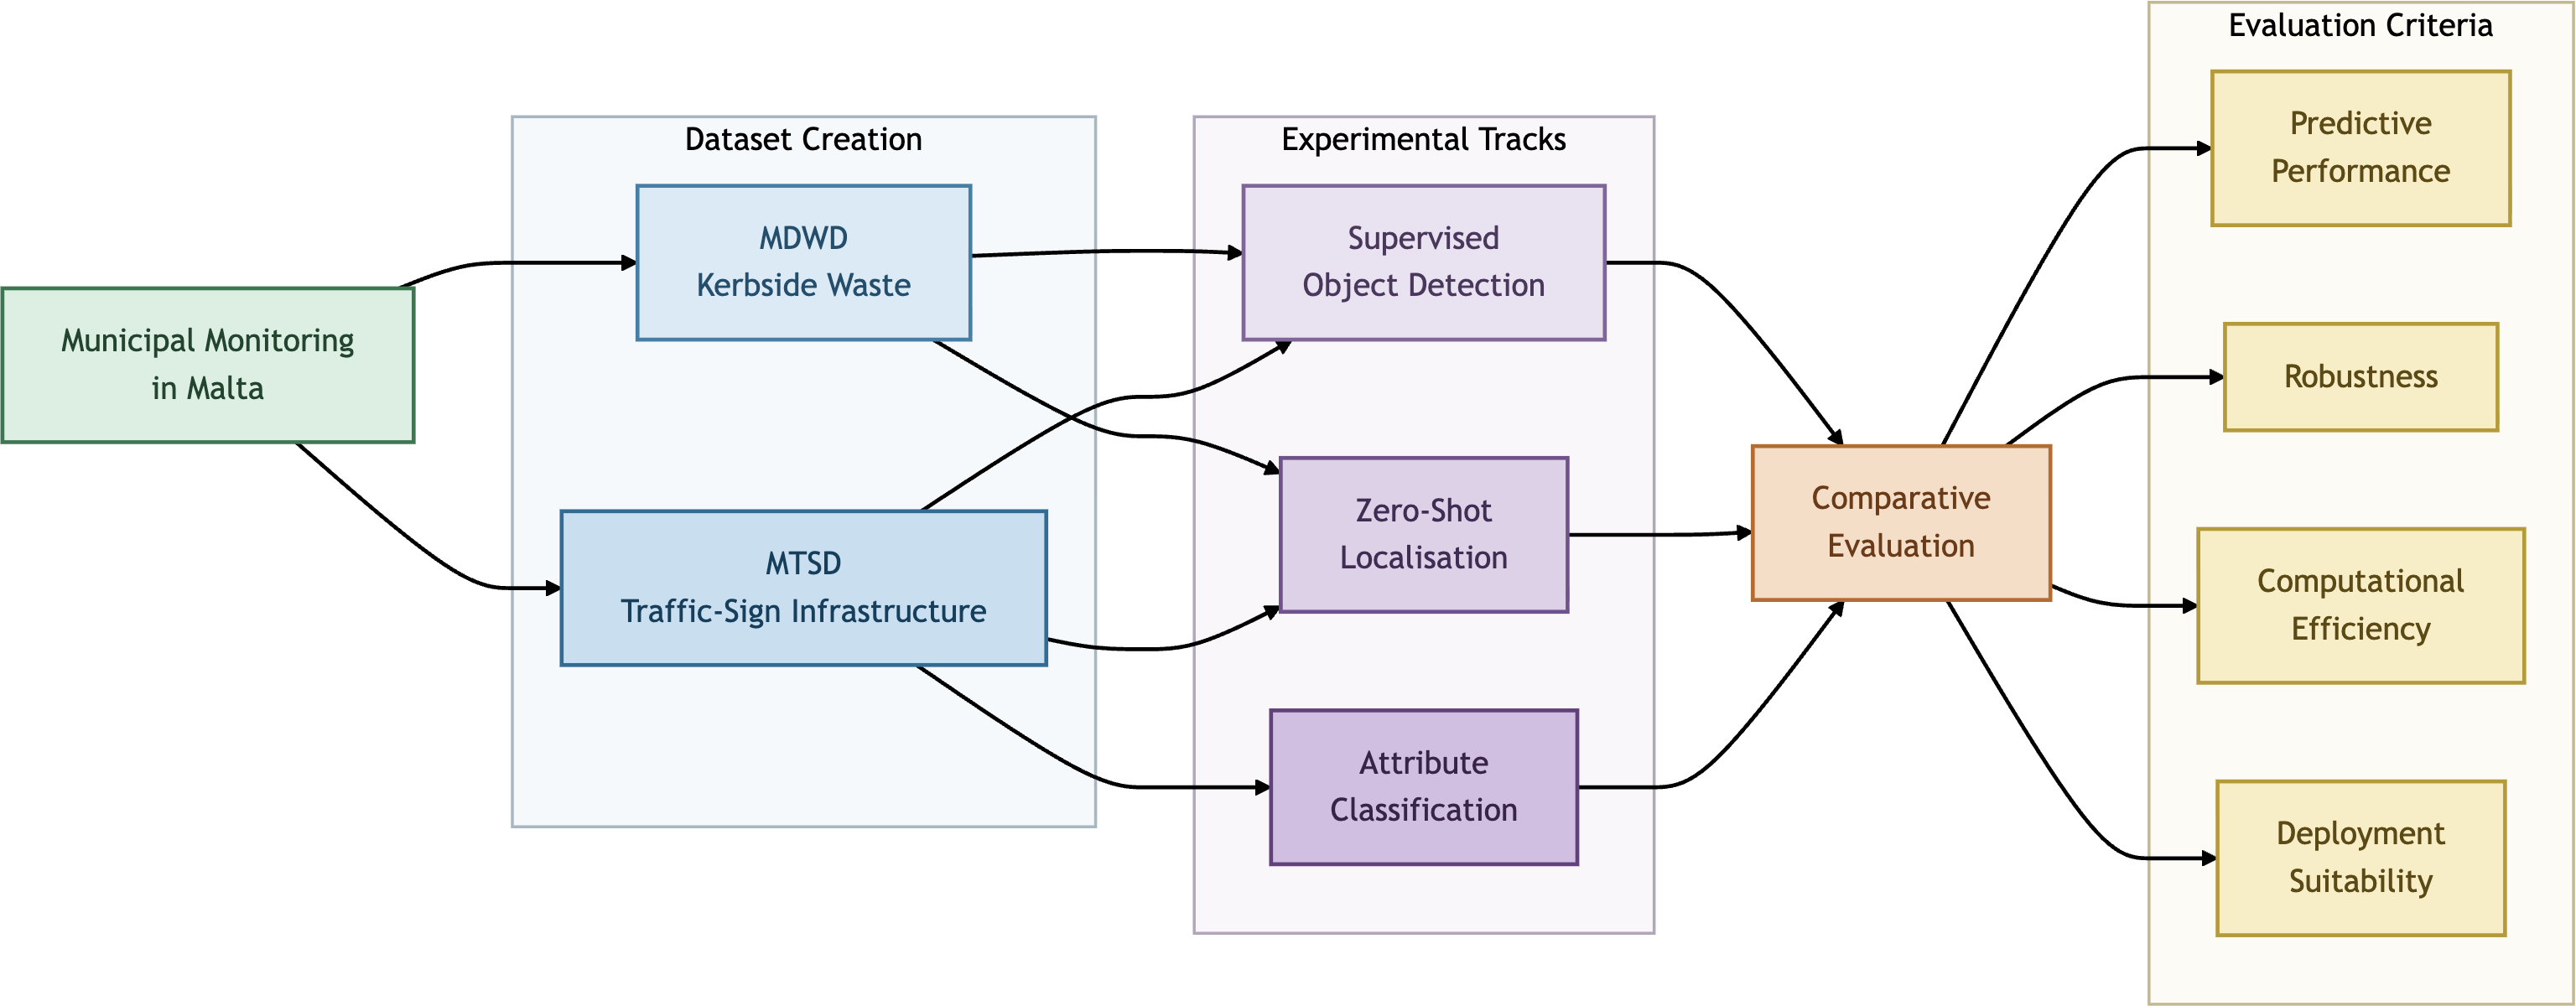
\includegraphics[width=\textwidth]{figures/ResearchApproach.png}
    \caption{Overview of the research approach, showing the relationship between the Maltese municipal-monitoring datasets, experimental tracks and comparative evaluation criteria.}
    \label{fig:research-approach}
\end{figure}

\noindent The empirical study is organised into three complementary experimental tracks, as illustrated in Figure~\ref{fig:research-approach}. The first investigates supervised \gls{OD} across both datasets, comparing \gls{YOLO}-family detectors with a detection-transformer architecture under a common evaluation procedure. The second evaluates zero-shot object localisation using promptable localisation models and grounded \glspl{VLM}, applied without task-specific parameter optimisation and assessed against the same held-out \gls{GT} annotations. The third examines traffic-sign attribute classification using \gls{GT} object crops from the \gls{MTSD}. Pretrained visual representations are compared within a shared multi-head classification framework using frozen feature extraction, parameter-efficient adaptation and, where computationally feasible, full \gls{FT} to assess viewing angle, mounting type, physical condition and geometric shape.

Across the three tracks, evaluation considers predictive performance, robustness, computational efficiency and practical deployment suitability. The resulting framework therefore examines not only model performance, but also the trade-offs between perception paradigms and their suitability for the municipal-monitoring tasks considered.

\section{Aims and Objectives}
\label{sec:aims-objectives}
The primary aim of this dissertation is to evaluate the suitability of contemporary vision-based perception paradigms and transfer strategies for kerbside-waste and traffic-sign infrastructure monitoring in Malta. This aim is addressed through the following objectives:

\begin{enumerate}
    \item \textbf{Construct and characterise two Malta-specific street-level datasets}, by defining their taxonomies and annotation criteria, coordinating image acquisition and professional annotation, and quality-assuring the resulting \gls{MDWD} for kerbside \gls{MSW} detection and the \gls{MTSD} for traffic-sign infrastructure monitoring. Both provide verified object-level annotations, with \gls{MTSD} instances additionally annotated for viewing angle, mounting type, physical condition and geometric shape.
    
    \item \textbf{Train and comparatively evaluate supervised detectors}, by training \gls{YOLO}11, \gls{YOLO}\\12, \gls{YOLO}26 and \gls{RF-DETR} on both datasets within a shared experimental framework, with framework-specific training differences recorded explicitly. Performance is quantified using detection, robustness and computational-efficiency measures, with controlled \gls{MTSD} experiments additionally assessing the effects of model scale, data augmentation and input resolution.

    \item \textbf{Quantify the effectiveness of zero-shot object localisation}, by evaluating \gls{SAM}~3, \gls{SAM}~3.1, LocateAnything and Cosmos Reason2 against common held-out \gls{GT} annotations without task-specific parameter optimisation. Localisation performance, sensitivity to prompt formulation and per-image inference cost are quantified, using controlled prompt variants where applicable, and compared with supervised \gls{OD}.
     
    \item \textbf{Compare transfer strategies for traffic-sign attribute classification}, by evaluating frozen feature extraction, \gls{LoRA}-based adaptation and full \gls{FT}, where computationally feasible, across \gls{DINO}v3, \gls{VJEPA}~2.1, ConvNeXt and LingBot-Vision within a common multi-head classification framework. Performance and computational requirements are quantified across viewing angle, mounting type, physical condition and geometric shape to identify the most effective representation--transfer strategy combinations for the \gls{MTSD}.

\end{enumerate}

\newpage
\noindent The conclusions drawn from these objectives are restricted to the two Maltese monitoring domains and datasets considered in this dissertation. Differences in dataset coverage, model characteristics and experimental conditions are therefore explicitly considered when interpreting the results, rather than treating the findings as universal comparisons between the underlying model families.

\section{Document Structure}
\label{sec:document-structure}
The remainder of this dissertation is organised into four chapters: \medskip

\noindent \textbf{\hyperref[ch:bg-lit]{Chapter 2 -- Background and Literature Review}} establishes the municipal and technical context of the study. It introduces the Maltese monitoring setting and the datasets used in this research, before reviewing related work and the \gls{CV} approaches relevant to the three experimental tracks. \medskip

\noindent \textbf{\hyperref[ch:methodology]{Chapter 3 -- Methodology}} describes the experimental framework and dataset preparation, together with the methods used for supervised detection, zero-shot localisation and traffic-sign attribute classification. \medskip

\noindent \textbf{\hyperref[ch:evaluation]{Chapter 4 -- Evaluation}} presents and analyses the experimental results, comparing the investigated approaches across the established evaluation dimensions and examining their principal failure modes. \medskip

\noindent \textbf{\hyperref[ch:conclusion]{Chapter 5 -- Conclusion}} consolidates the findings in relation to the dissertation aims and objectives, summarises the principal contributions and limitations, and identifies directions for future research.

\noindent\rule{\linewidth}{0.3pt}